O objetivo deste trabalho é desenvolver um software embarcado em um Raspberry Pi
equipado com módulo de câmera que seja capaz de reconhecer veículos, contá-los e
identificá-los baseando-se em sua placa. Todo o processamento deve acontecer em
tempo real com base nas imagens da câmera captadas no momento. A informação
coletada e processada deve ser enviada para um servidor que possa utilizar estes
dados em tempo real.

O fluxo esperado do software é o seguinte. O computador Raspberry pi ficará
postado em uma rota de fluxo frequente de carros. Ele ficará posicionado de
maneira que consiga capturar imagens das placas em boa qualidade com sua câmera.
Será nescessário o módulo de câmera e de bateria, ou haver uma fonte de energia
por perto. Ao capturar as imagens, o computador irá processá-las localmente,
seguindo os passos do reconhecimento de placas e contagem de carros.  Após
obtida, a informação será enviada para um servidor simples que irá armazená-la.
Para o envio das informações, o computador também precisará estar equipado com
algum módulo de internet.

O trabalho será realizado em etapas, tendo como objetivo intermediário conseguir
fazer o reconhecimento e a contagem dos carros, e como objetivo final a
identificação das placas.

\section{Raspberry Pi}
\label{sec:raspi}

Raspberry Pi é um computador construído em uma placa de circuito do tamanho de
um cartão de crédito desenvolvido pela Raspberry Pi
Foundation\footnote{https://www.raspberrypi.org/}.

\section{OpenCV}
\label{sec:opencv}

OpenCV (\emph{Open Source Computer Vision Library}) é uma biblioteca \emph{open
source} de visão computacional e aprendizado de máquina. Contém mais de 2500
algoritmos otimizados nessas áreas, incluindo algoritmos clássicos e recentes. A
biblioteca é escrita nativamente em C++, e dispõe de interfaces para C, C++,
Python, Java e MATLAB, suportando os sistemas operacionais Windows, Linux,
Android e Mac OS.\footnote{http://opencv.org/}

\section{OCR}
\label{sec:ocr}

Reconhecimento Ótico de Caracteres (\emph{Optical Character Recognition}, OCR)
consiste da conversão de textos em formato de imagem para o formato reconhecido
por máquina. É o método mais eficiente para fazer o processamento de imagem para
texto.~\cite{mohit2015designing}

Uma ferramenta conhecida de OCR é o
Tesseract\footnote{https://github.com/tesseract-ocr/tesseract}. É uma ferramenta
\emph{open source} de reconhecimento ótico de caracteres que suporta múltiplas
línguas.  É essencialmente um algoritmo de comparação de \emph{templates}, e as
amostras de caracteres podem ser auto-treinados.~\cite{ho2016intelligent}

\section{Placa de Transito Brasileira}
\label{sec:placabr}

Segundo o código de transito brasileiro~\cite{brasil1997lei}, todos os veículos
são identificados por meio de placas dianteira e traseira. Elas são
identificadas por uma tarja na parte superior contendo a sigla do estado e o
nome do município, e pelo código de identificação único, composto por três
letras, seguidas por quatro digitos, separados por um hífen.

Veículos particulares, de aluguel, oficial, de experiência, de aprendizagem e de
fabricante tem suas dimensões de 130mmx400mm e altura dos caracteres de 63mm.
Caso a placa não caiba no receptáculo ela pode ser reduzida em até 15\%. As
placas de motocicleta, motoneta, ciclomotor e triciclos autorizados tem
dimensões de 136mmx187mm e altura de caracteres de 42mm. Imagem das placas com
suas dimensões podem ser vistos nas figuras~\ref{fig:placa_carro}
e~\ref{fig:placa_moto}.

\begin{figure}[H]
		\centering
		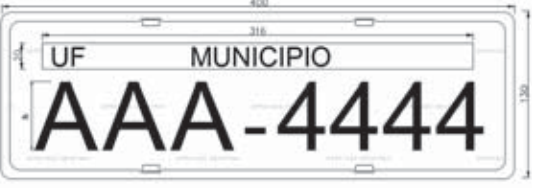
\includegraphics[width=88mm]{placa_carro.png}
		\caption{Placa de um carro}
		\label{fig:placa_carro}
\end{figure}

\begin{figure}[H]
		\centering
		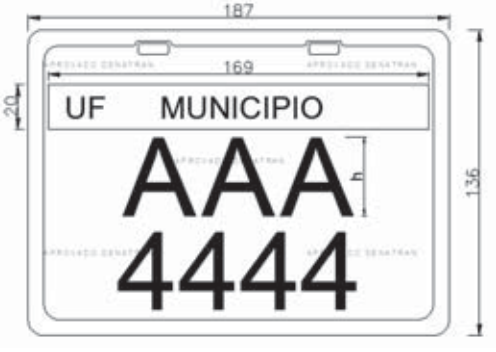
\includegraphics[width=88mm]{placa_moto.png}
		\caption{Placa de uma moto}
		\label{fig:placa_moto}
\end{figure}

A tipologia dos caracteres das placas utiliza a fonte
Mandatory~\ref{fig:tipografia}, e as placas de categorias diferentes de veículos
são diferenciadas pelas suas cores na tabela~\ref{tab:placa_cores}.

\begin{figure}[H]
		\centering
		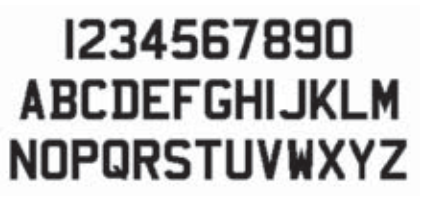
\includegraphics[width=88mm]{fonte.png}
		\caption{Tipografia das placas}
		\label{fig:tipografia}
\end{figure}

\begin{table}[]
\centering
\label{tab:placa_cores}
\caption{Cores das placas automotivas}
\begin{tabular}{|l|l|l|}
\hline
\textbf{Categoria do Veículo}                                               & \textbf{Cor de Fundo} & \textbf{Cor de Caracteres} \\ \hline
Particular                                                                  & Cinza                 & Preto                      \\ \hline
Aluguel                                                                     & Vermelho              & Branco                     \\ \hline
Experiência/Fabricante                                                      & Verde                 & Branco                     \\ \hline
Aprendizagem                                                                & Branco                & Vermelho                   \\ \hline
Coleção                                                                     & Preto                 & Cinza                      \\ \hline
Oficial                                                                     & Branco                & Preto                      \\ \hline
Missão Diplomática                                                          & Azul                  & Branco                     \\ \hline
Corpo Consular                                                              & Azul                  & Branco                     \\ \hline
Organismo Internacional                                                     & Azul                  & Branco                     \\ \hline
Corpo Diplomático                                                           & Azul                  & Branco                     \\ \hline
\begin{tabular}[c]{@{}l@{}}Organismo Consular/\\ Internacional\end{tabular} & Azul                  & Branco                     \\ \hline
\begin{tabular}[c]{@{}l@{}}Acordo Cooperação\\ Internacional\end{tabular}   & Azul                  & Branco                     \\ \hline
Representação                                                               & Preto                 & Dourado                    \\ \hline
\end{tabular}
\end{table}

\section{Implementação}
\label{sec:implementacao}

Segundo Ahmad et al.~\cite{ahmad2015automatic}, o reconhecimento de placas
automotivas requer três passos, a localização da placa, a separação dos
caracteres e o reconhecimento dos caracteres. Para a localização da placa e
separação dos caracteres serão utilizados a biblioteca OpenCV e a linguagem de
programação C, C++ ou Python. O motivo da escolha dessas linguagens se dá porque
são as linguagens mais usadas para OpenCV, a melhor abordagem ainda será
analisada. Para o reconhecimento dos caracteres será estudada a possibilidade de
utilizar o software Tesseract ou criar uma solução própria. As escolhas a serem
feitas tem como objetivo maximizar os resultados ao final do trabalho, tentando
criar um balanço entre facilidade de implementação e qualidade do
reconhecimento.

O algoritmo a ser implementado neste trabalho utilizará como base as técnicas de
identificação e detecção de Wafy e Madbouly~\cite{wafy2016efficient}, pois foram
os resultados mais promissores encontrados em primeira pesquisa.

